\chapter{step} \label{stepN}

\section{Introduction}

\txs{} provides commands for randomly stepping through a model; however, it may be possible to do this more efficiently when a model is in LPE form.
This hypothesis has been put to the test by developing dedicated stepper functionality.

Early results of the LPE stepper showed equal to worse performance.
The LPE stepper was therefore extended with a preparatory step in which `possible successors' are calculated.
Making use of the extra information, the LPE stepper frequently outperforms the original \txs{} stepper.

\section{Formal background}

\subsection{Possible successors}

Consider summands $s_\alpha$ and $s_\beta$, referencing their elements conform \ref{summandelements}.
Summand $s_\beta$ is said to be a \emph{possible successor} of $s_\alpha$ if the following expression \emph{could be} satisfiable:
\begin{align*}
g_\alpha \land {g_\beta}[v \rightarrow q(v) \;|\; v \in \varsof{g_\beta} \setminus P][p \rightarrow v_\alpha(p) \;|\; p \in P]
\end{align*}

where $q(v)$ is a bijective function that relates variable $v$ to a fresh variable.

\section{Algorithm}

\subsection{Preparation}

The algorithm computes all possible successors for each summand.
(In actuality, the algorithm can compute possible successors of a sequence of summands of arbitrarily chosen length $n \geq 1$.
Unsurprisingly, when choosing $n > 1$ cases in which the costs to compute possible successors are prohibitive are far from uncommon.)

\subsection{Step}

Let $\Sigma$ be a set of tuples $\shPair{\sigma}{h}$ in which $\sigma$ is a model state and $h$ is the history of summands that led to $\sigma$.
Initially, $\Sigma = \{\;\shPair{\sigma_0}{[\;]}\;\}$ where $\sigma_0$ is the initial state as defined by the LPE model.

\subsubsection{1. Compute \istep{}-closure}

Let $T$ be the set of all \istep{} summands of the LPE.
Apply each $t \in T$ to each $\sigma \in \Sigma$.
Any new state $\sigma'$ that is produced by some $t \in T$ is added to $\Sigma$ as $\shPair{\sigma'}{[t]}$.
This is repeated until $\Sigma$ no longer changes.

\subsubsection{2. Find an enabled summand}

Let $\overline{T}$ be the set of all non-\istep{} summands of the LPE.

Consider the summands in $\overline{T}$ in a random order, and let the summand under consideration be $u$.
Determine whether there is a $\shPair{\sigma}{[t]} \in \Sigma$ so that $u$ is enabled when the current state is $\sigma$.
If so, find a \emph{random} variable-to-value mapping $C$ so that $g_u[\; x_u(i) \mapsto C(i) \;|\; i \in [1,\cdots{},m_u] \;]$ holds when the current state is $\sigma$.
Remember $u$ and $C$ (in particular, add it to the random trace that is being constructed) and continue with the next part of the algorithm immediately.

If no $u$ and $C$ can be found, the algorithm reports a deadlock and terminates.

It is also possible that the maximum length of the trace has been reached, in which case the algorithm also terminates.

\subsubsection{3. Determine next states}

In this part of the algorithm, the new value of $\Sigma$ is computed.

For each $\shPair{\sigma}{[t]} \in \Sigma$, look up the possible successors of $t$.
For each possible successor $p$ of $t$, check if the channel of $p$ is the same as the channel of $u$ (that is, if $c_{p} = c_{u}$), then check if $g_p[\; x_p(i) \mapsto C(i) \;|\; i \in [1,\cdots{},m_p] \;]$ holds when the current state is $\sigma$:
\begin{itemize}
\item If the equation holds, apply the summand $p$ to $\sigma$ to find the next state $\sigma'$.
Add $\shPair{\sigma'}{[p]}$ to the new value of $\Sigma$.
\item If the equation does not hold, nothing is added to the new value of $\Sigma$.
\end{itemize}

\clearpage
\section{Benchmark results}

The performance of the LPE stepper has been compared to the performance of the original stepper of \txs{}.
Because the LPE stepper only works for LPEs, the performance of the original stepper has been measured for both unchanged input models and linearized input models.

Figure~\ref{steppers:fig} shows two bars per model: the blue bar is the time that the original stepper of \txs{} required to generate a 100-step trace from the linearized input model as a fraction of $\Delta t$, the time that the original stepper of \txs{} required to generate a 100-step trace from the unchanged input model.
Similarly, the yellow bar is the time that the LPE stepper required to generate a 100-step trace from the linearized input model (obviously, this is a precondition on the input of the LPE stepper) as a fraction of $\Delta t$.
The figure also includes the range of the standard deviation.

\begin{figure}[!ht]
\begin{center}
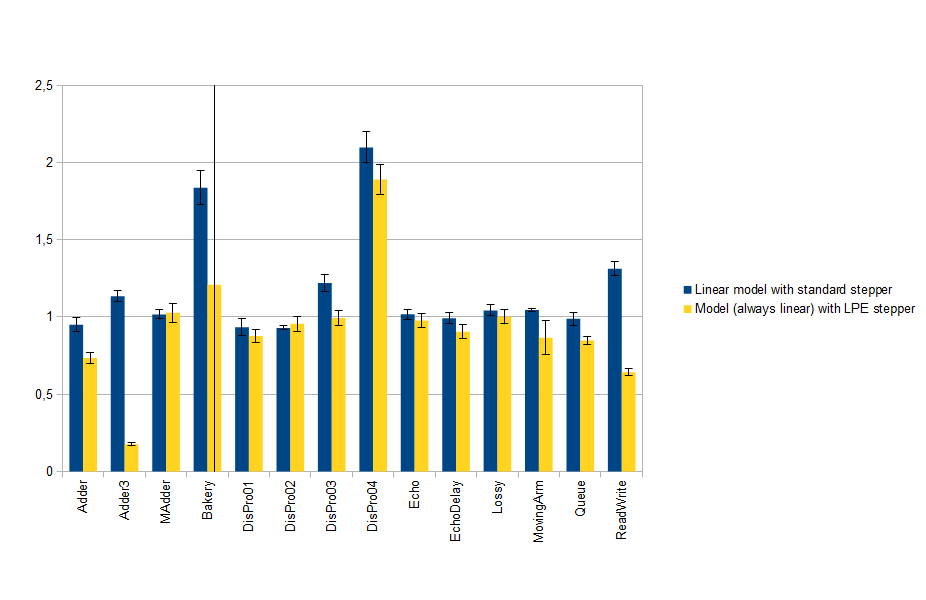
\includegraphics[width=1\linewidth]{charts/steppers-comparison}
\caption{Relative performance of different steppers}
\label{steppers:fig}
\end{center}
\end{figure}

As can be seen in the figure, for 7 out of 14 models the deviation ranges of the measured times overlap, and so we cannot conclude a performance improvement.
For all other models, however, the LPE stepper actually outperforms the original stepper, even though the performance is only impressive for the Adder, Adder3, and ReadWrite models.

The Bakery model has a very large standard deviation.
This deviation results from the long preparatory step that the model requires -- it is quite a large model -- and from the way in which benchmark measurements were taken:
\begin{enumerate}
\item The LPE stepper was instructed to generate a 100-step trace.
The required time $\Delta t _ {100}$ was measured.
\item The LPE stepper was instructed to generate a 0-step trace.
The required time $\Delta t _ {0}$ was measured.
\item $\Delta t$ was computed by subtracting $\Delta t _ {0}$ from $\Delta t _ {100}$.
\end{enumerate}
Naturally, the impact of the deviation in $\Delta t _ {0}$ becomes stronger as the value of $\Delta t _ {0}$ increases relative to $\Delta t _ {100} - \Delta t _ {0}$.

